\subsection{Hardware stack}
In principle, any device with computing, storage, and network connectivity could act as a fog node~\cite{ciscoFog}. Additionally, fog nodes should be able to be distributed geographically, to cope with different network types, to be cheap and easy to replicate. We chose to work with Raspberry Pi 3b+ (Quad-core 64-bit ARM processor, 1GB of RAM, 32GB of storage) single-board computers as standard devices. However, as such devices are rather limited in terms of processing capabilities (mostly related to the little amount of RAM available), we decide to build a small cluster of five Raspberry Pi 3b+, and use such cluster as fog node hardware platform. In Figure~\ref{fig:fridge} we present two images of the cluster, which we refer to as 'fridge'.
 % (Quad-core 64-bit ARM processor, 1GB of RAM, 32GB of storage) single-board computers as a cluster of hardware device \notedb{fig or pic of HW setup maybe}. We used D-Link DWR-921 router (with OpenWRT installed) as Wi-Fi Access Point for the clusters.
% }
\begin{figure}[htbp]
\centerline{
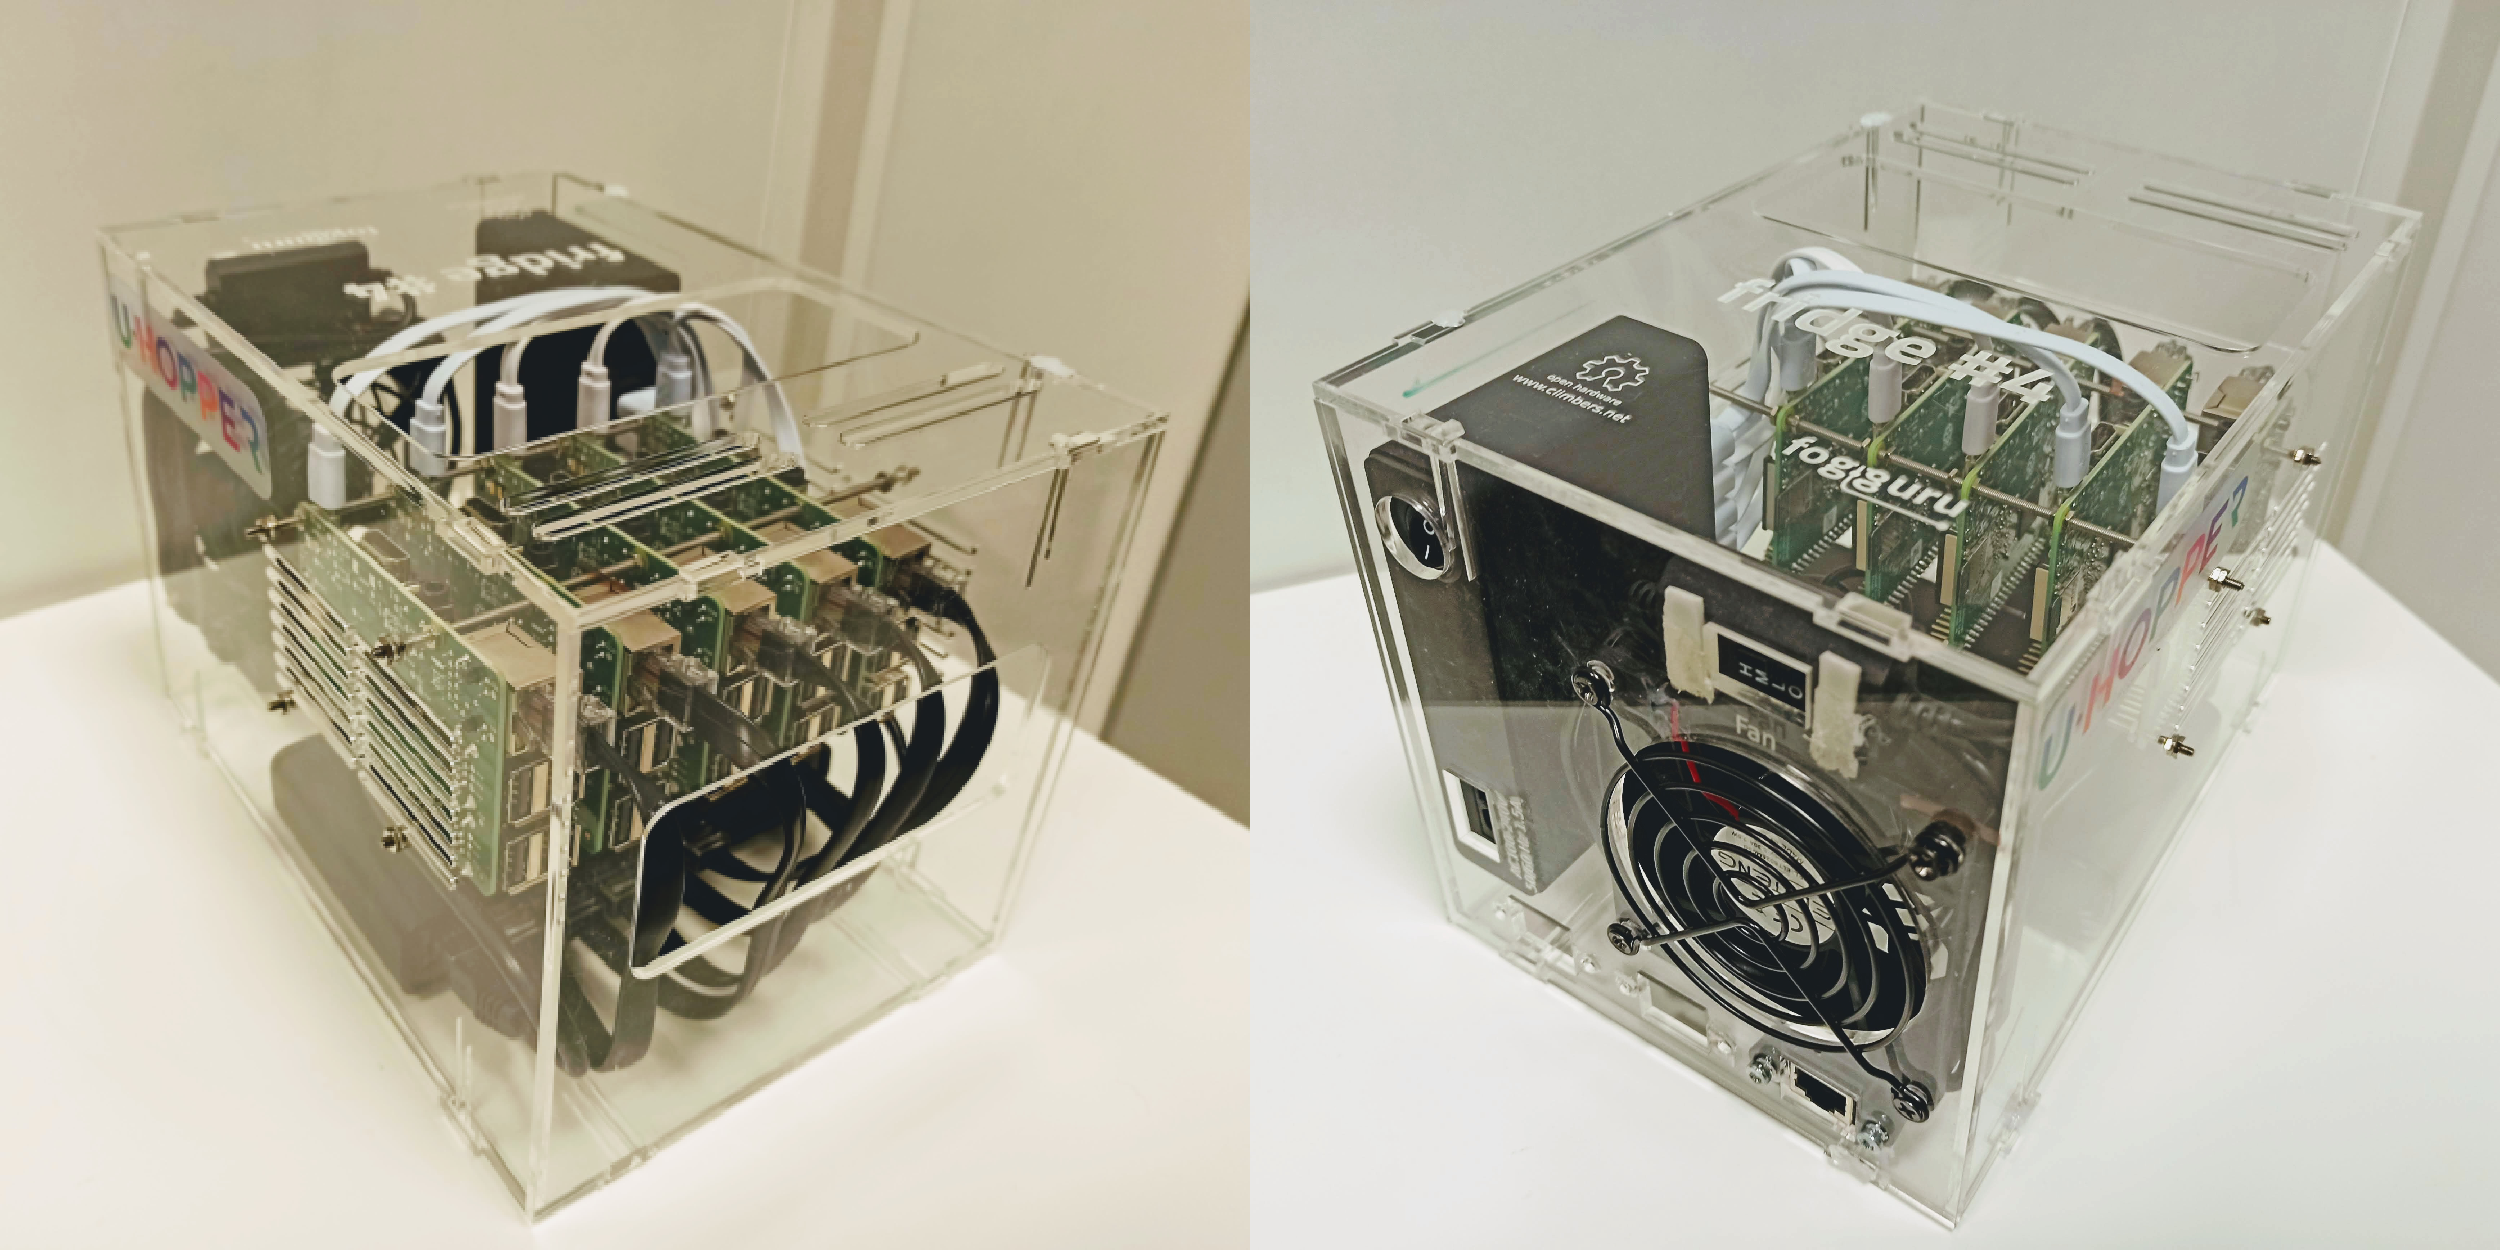
\includegraphics[width=1\linewidth]{figures/fog_pic.pdf}}
\caption{The FogGuru hardware platform (cluster of 5 Raspberry Pi 3b+), commonly referred to as 'fridge'.}
\label{fig:fridge}
\end{figure}


\subsection{Platform architecture}
The FogGuru platform high-level architecture is represented in Figure~\ref{fig:node-arch}. It is consistent with standard architectures in edge/fog computing (see~\cite{de2018distributed}) and in data processing pipelines~\cite{ismail2019manufacturing}. Data from the IoT tier gets ingested through a suitable queuing system, from where it is fetched to be (stream-)processed. Intermediate results may be fed back to the message queueing system and/or stored persistently, depending on the expected usage. Processed data (represented as a stream) is pushed to the cloud tier for further aggregation/analysis. The operations of the stream processing engine are monitored, and relevant log data (or basic analytics) are also pushed to the cloud tier in batches.
% indicated the key components in real-time data processing architecture. And they can be simplified, as shown in Figure~\ref{fig:node-arch}.

\begin{figure}[htbp]
\centerline{
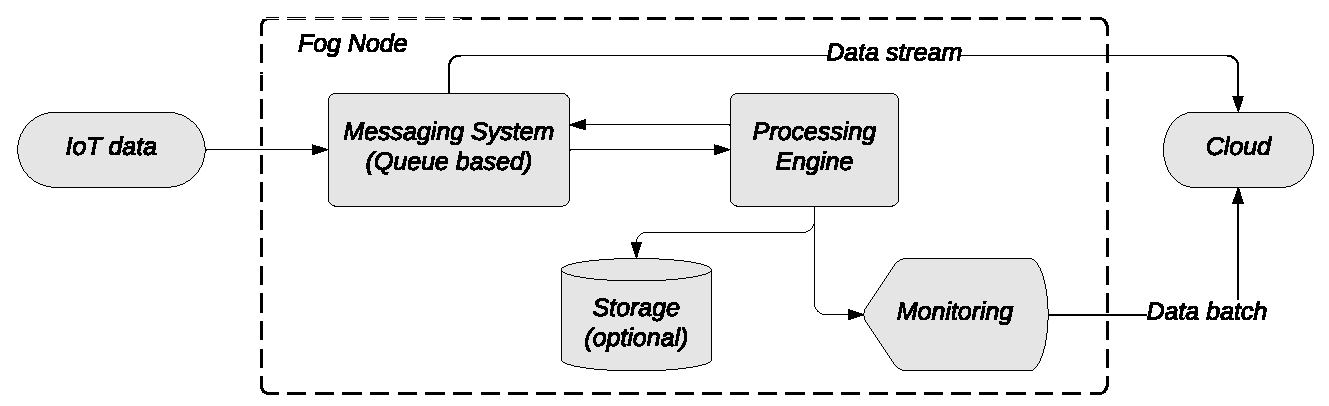
\includegraphics[width=1\linewidth]{figures/fog_components.pdf}}
\caption{The FogGuru platform architecture.}
\label{fig:node-arch}
\end{figure}

The choice of appropriate technologies/frameworks for implementing such an architecture plays a critical role. Here is a brief description of our design choices.
% Choosing a suitable software stack for the resource-constrained environment is crucial for fog application deployment.
\paragraph*{Messaging System}
Message Queue Telemetry Transport (MQTT) is a lightweight publish-subscribe network protocol widely used in IoT applications, and better suited for fog applications than more powerful (but resource-hungry) cloud frameworks (such as, e.g., Apache Kafka). We decided to use the open-source Mosquitto\footnote{https://mosquitto.org/} MQTT broker as our message handler.

\paragraph*{Processing}
Stream Processing Engines (SPEs) represent a good paradigm for Fog computing applications because of their extensive set of features, including support for event-driven, data pipeline, and data analytics applications. Constrained resources is also here an aspect to cater for; the literature includes surveys on how various SPEs perform in a fog environments~\cite{lee2017data,zeuch2019analyzing}. We decided to use Apache Flink\footnote{https://flink.apache.org/} as our SPE of choice. Apache Flink is a distributed, open-source, stream processor with intuitive and expressive APIs to implement stateful stream processing applications.

\paragraph*{Monitoring}
We used Prometheus\footnote{https://prometheus.io/} and Grafana\footnote{https://grafana.com/} for computing real-time performance indicators based on Apache Flink metrics APIs.
% as a time series Database for recording real-time metrics.
 % and Grafana as the web interface for analysis and visualization./notedm{remove reference to Grafana and focus on storage here, for the monitoring part leave it empty (we don't have it actually..)}

\paragraph*{Containerization}
Using container orchestration is mandatory for deploying fog applications at scale. It packages software components and their dependencies and deploys them in a standardized way. There are studies about performance evaluation of container orchestrators in Fog environment~\cite{hoque2017towards}. We used the Docker\footnote{https://www.docker.com/} ecosystem for its portable deployment.
